\documentclass{article}      % use "amsart" instead of "article" for AMSLaTeX format
\usepackage{graphicx}               % Use pdf, png, jpg, or eps§ with pdflatex; use eps in DVI mode
                                % TeX will automatically convert eps --> pdf in pdflatex   
\usepackage{caption}
\usepackage{subcaption}
\captionsetup{justification=raggedright,singlelinecheck=false}

\usepackage{amsmath}
\usepackage{amsthm}
\usepackage{amsfonts}
\usepackage{verbatim}
\usepackage{bm}
\usepackage{multicol}
\usepackage[switch]{lineno}
\usepackage{hyperref}

\usepackage{icml2025}


\newcommand{\cov}{\mathrm{cov}}

\usepackage{setspace}

\begin{document}
\twocolumn[
\icmltitle{Cumulant Generating Function Networks for Adaptation of Neural Network Statistics}

\begin{icmlauthorlist}
\icmlauthor{Luke Rast}{yyy}
\end{icmlauthorlist}

\icmlaffiliation{yyy}{Department of XXX, University of YYY, Location, Country}
\icmlcorrespondingauthor{Luke Rast}{first1.last1@xxx.edu}

\vskip 0.3in
]
\printAffiliationsAndNotice{}


\begin{abstract}
  Neural network performance suffers when input statistics differ between training and application data.
  The cumulant generating function provides access to classical methods for detecting and adapting to distributional changes.
  We learn cumulant generating functions that capture the statistics of internal layers in a trained neural network, and apply them to change detection and adaptation of the network.
  Specifically, we learn an input convex neural network representation of the cumulant generating function, and use saddlepoint approximation for change detection and exponential tilting for adaptation.
  Taking advantage of the neural network representation, we also learn a cumulant generating function representation of target-conditional distributions, allowing for application of Bayesian inference under label shift.
  We demonstrate these methods on simple examples.
\end{abstract}


\section{Introduction and background}

Machine learning models in applications often face input statistics that differ from the datasets that they were trained and tested on, resulting in decreased performance \cite{recht_imagenet_2019,koh_wilds_2021}.
\textit{Domain adaptation} addresses this problem by detecting these distributional shifts and adapting the models to them.
In neural network models, domain adaptation techniques often detect changes based on the distribution of model outputs \cite{lipton_detecting_2018,garg_leveraging_2022}, and perform adaptation by finetuning with importance weights that reflect probability of the training data in the new distributional context \cite{lipton_detecting_2018,maity_understanding_2023}.
Both of these steps require a model of how  the neural network activity is distributed under different input conditions.
In this work, we model the distribution of network activity using the cumulant generating function, which is very well suited to both change detection and adaptation.

The \textit{cumulant generating function} (CGF) of a random variable, $x$, is given by
\begin{equation}
  A(\theta) = \log \mathbb{E}_x[\exp(\theta^T x)]. \label{def:cgf}
\end{equation}
It is the logarithm of the moment generating function, and, when it exists, provides a unique representation of the distribution of $x$.
Importantly, the CGF is guaranteed to be \textit{convex} \cite{barndorff2014information}.
We use the CGF to represent the distribution of network activity. 

One application of the CGF is constructing families of \textit{exponentially tilted} probability distributions \cite{morris_natural_1982,morris_unifying_2009}.
Starting from a baseline distribution $h(x)$, with cumulant generating function $A(\theta)$, exponential tilting produces the family
\begin{equation}
  p(x | \theta) = h(x) e^{\theta^T x - A(\theta)}. \label{def:exponential_tilt}
\end{equation}
This is a natural exponential family of distributions, each of which modifies the base measure $h(x)$ by concentrating the probability density along different directions to different extents.
The CGF gives the cumulant generating functions for every member of the tilted family
\begin{equation}
  A_\theta(\phi | \theta) = A(\theta + \phi) - A(\theta) \label{eq:CGF_family}
\end{equation}
Thus, the mean of any distribution in the family is given by the Jacobian of the CGF,
\begin{equation}
  \mu(\theta) = \nabla_\theta A(\theta) \label{eq:cgf_jacobian}
\end{equation}
while the Hessian gives the covariance matrix, and so forth \cite{barndorff2014information}.
Due to convexity, there is a one-to-one relationship between $\theta$ and $\mu$.
We use exponential tilting to model neural network activity in different input conditions, which we use for adaptation.

Another application of the CGF is saddlepoint approximation \cite{daniels_saddlepoint_1954,barndorff-nielsen_edgeworth_1979}.
Given a distribution $h(x)$, with cumulant generating function $A(\theta)$, the saddlepoint approximates the distribution of sample means by
\begin{equation}
  p(\mu; n) \approx \left( \frac{n}{2\pi} \right)^{d\frac{d}{2}} |V(\mu)|^{-1/2} \exp(-n I(\mu)). \label{def:mean_density}
\end{equation}
Where $\mu$ is the sample mean of $n$ samples in $d$ dimensions, $V(\mu)$ is covariance matrix (given by the Hessian of the CGF), and $I(\mu)$ is the rate function.
The \textit{rate function} is the Legendre transform of the cumulant generating function
\begin{equation}
  I(\mu) = \sup_{\theta}(\mu^T \theta  - A(\theta) ), \label{eq:legendre_transform}
\end{equation}
and corresponds to the rate function in large deviations theory, by Cramer's Theorem \cite{dembo2009large}.
The saddlepoint approximation becomes asymptotically tight as the number of datapoints increases \cite{iltis_sharp_1995,chaganty_multidimensional_1986}, but remains quite accurate at lower sample sizes \cite{davison_saddlepoint_1988,ronchetti_empirical_1994} as well.
We use the saddlepoint approximation to perform change detection.

In summary, the cumulant generating function, gives access to two related functions, $A(\theta) \leftrightarrow I(\mu)$, the CGF and the rate function, related through Legendre duality.
Their arguments provide two related parameterizations $\theta \leftrightarrow \mu$ of the exponentially tilted family, corresponding to natural parameters $\theta$ and mean parameters, $\mu$.
Due to the duality, these are related by 
\begin{eqnarray}
  \mu = \nabla_\theta A(\theta) & \theta = \nabla_\mu I(\mu). \label{eq:duality_relations}
\end{eqnarray}
The function pair allows detection of changes in sample means, through the saddlepoint distribution~(\ref{def:mean_density}), and adaptation of the distribution that models the the sampling process, through exponential tilting~(\ref{def:exponential_tilt}).

We apply these dual functions to the twin problems of change detection and adaptation.
On one side of this duality, the rate function $I(\mu)$, gives the probability density over the mean of many samples.
We use this density to detect changes in the statistics of the world.
On the other side of the duality, the cumulant generating function $A(\theta)$ provides the basis for a family of modified versions of environmental statistics.
We use this family to adapt to changes in the statistics of the world.
We capture both functions using a learned representation of the cumulant generating function, the \textit{CGF network}.

We apply this approach to illustrative examples, and to the activity of hidden layers of pre-trained classifier neural networks.
We show that CGF networks are able to capture both marginal and target-conditional distributions of neural network activity.
We show that marginal CGF networks give saddlepoint approximations that perform well at change detection, and exponential tilting weights that correctly up- and down- weight training points under label shifts.
We show that conditional CGF networks can be used directly for label inference and can fit shifted label distributions.


\section{Related work}

There is a large literature on domain adaptation \cite{kouw_introduction_2019}, as well as on change detection more broadly, and the related problems of anomaly detection \cite{pang_deep_2021}, change detection with single samples, and domain generalization \cite{gulrajani_search_2021}, which allows training sets from multiple environments.
Two special cases of domain adaption have received particular attention because they correspond to simple causal models for input and target generation \cite{scholkopf_causal_2012,zhang_domain_2013}.
Given inputs $x$ and targets $y$, \textit{label shift} assumes that $p(y)$ changes while $p(x|y)$ is constant, and \textit{covariate shift} assumes that $p(x)$ changes while $p(y|x)$ is constant.


Detection of distributional shifts is often performed by using statistical tests on some features of the input data.
This can be random feature embedding \cite{garg_unified_2020}, unsupervised dimensionality reduction techniques \cite{rabanser_failing_2019}, or features of the model itself.
\cite{lipton_detecting_2018} introduced black box shift detection, which uses the empirical frequencies of target outputs and the empirical confusion matrices (both from the training set) to approximate the output distributions.
Other feature of model outputs, like confidence \cite{hendrycks_baseline_2017} or entropy \cite{garg_leveraging_2022} have also been investigated for models that produce probability-like outputs.
Our approach also uses features of the learned classifier, in this case the distribution of internal activity of a neural network, to perform distribution shift detection.

Adaptation to distributional shifts has seen many approaches.
This includes retraining some network weights on a secondary task at application time \cite{sun_test-time_2020} and projecting novel input data toward the training set \cite{gao_back_2023}.
However, importance weighted empirical risk minimization, where importance weights are determined from application-time data is particularly common.
This approach has been investigated for covariate shift \cite{sugiyama_covariate_2007} using weights from Gaussian approximations to the data, label shift \cite{lipton_detecting_2018,garg_unified_2020} using weights from output distributions, as well as for general distributional shifts \cite{zhang_domain_2013,maity_understanding_2023}.
The recent work of \cite{maity_understanding_2023} assumed that distribution shifts could be modeled by exponential tilting of the training-set distribution, thereby giving importance weights via the exponential term in Equation~(\ref{def:exponential_tilt}).
We use the same exponential tilting approach here, albeit with the key differences that the sufficient statistics are layer activities in our baseline network, while parameter and normalization values are computed from the cumulant generating function networks.
On the Bayesian side, \cite{saerens_adjusting_2002} derived an expectation-maximization approach that could be used to fit label probabilities under label shift, which they use to modify posterior distributions.
\cite{alexandari_maximum_2020} showed that, given a neural network with calibrated outputs, this Bayesian approach to the label shift problem empirically outperforms importance weighted empirical risk minimization.



Our approach is similar in flavor to energy based modelling \cite{lecun_tutorial_2006}, which fits un-normalized log probabilities.
In fact, the cumulant generating function that we fit here is what is often called the free energy, and resembles the normalization factor in these models, which is intractable in many cases.
The distinguishing factor for this particular case is the fact the the model is like an exponential family, in that the parameters and inputs only interact linearly in the energy term.
This grants us tractability through the cumulant generating function interpretation.


A final important ingredient for our approach are input convex neural networks.
Introduced by \cite{amos_input_2017}, with later refinements to their architecture and weight initialization by \cite{hoedt_principled_2023}, these networks are guaranteed to produce convex functions of their inputs by using convex non-linearities, and enforcing positive weights in all but the first layer of the network.
These network were immediately put to use in energy based modelling \cite{amos_input_2017}, and have been used for probabilistic modelling in the context of optimal transport \cite{makkuva_optimal_2020,alvarez-melis_optimizing_2022}.


\section{Results}

We use a learned cumulant generating function to track the internal statistics of a neural network and to compare these internal statistics in novel environments.
Assume that we have a neural network, the \textit{classifier network} $\mathcal{N}_0$, that is trained for a classification task, mapping inputs, $x$, to target labels, $y$.
Given the trained network $\mathcal{N}_0$, we choose one hidden layer of the network, which we denote $T=T(x)$ to be our feature vector, and train a second neural network, which we call the \textit{CGF network} $A(\theta)$, to capture the statistic of $T(x)$ across inputs by reproducing its cumulant generating function. 
Combining $T(x)$ and $A(\theta)$ using exponential tilting (\ref{def:exponential_tilt}) gives an exponential family of distributions over $x$, with sufficient statistics $T(x)$ that are the features learned by $\mathcal{N}_0$.

\subsection{CGF networks}
We parameterize the CGF network using an input convex neural network \cite{amos_input_2017,hoedt_principled_2023}, which ensures that the learned CGF is convex, and that its derivatives can be evaluated by auto-differentiation.
We train the CGF network to reproduce the values of the empirical cumulant generating function (eCGF)
\begin{equation}
  \hat A(\theta) = \log \left( \frac{1}{N}\sum_{i} \exp(\theta^T T_i) \right), \label{def:empirical_CGF}
\end{equation}
which uses the empirical mean to evaluate the expectation in the CGF. 
This expression has previously been used as a CGF estimator for $n$ dimensional data \cite{davison_saddlepoint_1988,ronchetti_empirical_1994} in the context of saddlepoint approximation.

We train the CGF network by randomly sampling a variety of $\theta$ input values and training the network to produce the value of $\hat A(\theta)$ from expression (\ref{def:empirical_CGF}).
As show in Figure~\ref{fig:1a_CGF_Normal} for data with unit variance, the empirical CGF accurately captures the ground truth CGF at $\theta$ values that are close to zero.
However, it begins to diverge as $\theta$ moves farther from the origin, with limiting behavior that is linear rather than quadratic. 
The CGF network perfectly mimics the behavior of the eCGF.
However, evaluating the corresponding probability density (as described below), we recover a quite accurate approximation of ground truth, Figure~\ref{fig:1a_CGF_Normal}.
This shows that it is most important to capture the values of the empirical CGF at inputs close to the origin.
Because of this, we always sample training values of $\theta$ that are concentrated around the origin (regardless of the dimensionality).
We also preprocess data coming into the CGF network to have zero mean and unit variance, across all dimensions. 
See Section~\ref{sec:network_architecture} for full details of our CGF network, training, and preprocessing.

\begin{figure}[tb]
  \centering
  \begin{subfigure}[t]{0.5\textwidth}
    \centering
    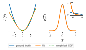
\includegraphics[]{figures/figure1a.pdf}
    \caption{Univariate standard normal distribution, 5k samples. Left: CGF, Right: pdf, Inset: pdf zoomed around $x=4.9$}
    \label{fig:1a_CGF_Normal}
  \end{subfigure}
  \begin{subfigure}[t]{0.5\textwidth}
    \centering
    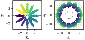
\includegraphics[]{figures/figure1b.pdf}
    \caption{Class-conditional distribution, 4k samples. Left: scatterplot of the data, colored by target, Right: scatter plot of parameter samples $\theta(y) + \phi$ , colored by conditional eCGF value, contours show the conditional CGF network fits}
    \label{fig:1b_conditional_CGF}
  \end{subfigure}

  \caption{Learned Cumulant generating functions of simple distributions. (a): CGF network fits to univariate normal distribution (b): conditional CGF network fits to bivariate, target conditional normal distribution}
  \label{fig:1_CGF}
\end{figure}


One key advantage of the CGF network representation of $A(\theta)$ is that we can also evaluate the dual rate function $I(\mu)$ and transform $\theta \leftrightarrow \mu$ between equivalent values of the natural and moment parameters.
Following equation~(\ref{eq:duality_relations}), we compute the mean parameters $\mu(\theta)$ using the Jacobian of the neural network. 
Evaluation of $I(\mu)$ and $\theta(\mu)$ both come down to evaluating the Legendre transform (Eq.~\ref{eq:legendre_transform}), which we do by directly solving the optimization problem using gradient descent in $\theta$.
The resulting optimal input gives $\theta(\mu)$, while the optimal value is $I(\mu)$.
Note that more sophisticated optimization approaches are also available.

We use the rate function $I(\mu)$ and the determinant of the Hessian, ${V(\mu) = \bm{H}[A](\theta(\mu))}$, to compute the saddlepoint approximation of the probability density, Eq.~(\ref{def:mean_density}).
Figure~\ref{fig:1a_CGF_Normal} shows this approximate probability density for univariate Gaussian data.
The approximation is quite good, but shows a characteristic deviations in the tails, highlighted in the inset:
the approximate pdf falls sharply to zero beyond a cut-off point. 
This is the result of the fact that the empirical CGF becomes linear at large values, meaning that the Legendre transform diverges to infinity for $\mu$ values exceeding the maximum (or minimum) slope.
The linearity of the eCGF, in turn, can be understood from Equation~(\ref{def:empirical_CGF}): as $\theta$ gets large, the sum is increasingly dominated by only the term with the largest $T_i$ value.
The result is that the limiting slopes, and therefore the cut-off values of the approximate density, are dominated by the extreme values in the training data: the approximate probability decays exponentially outside the range of observed datapoints.



\subsection{Conditional CGF networks}

Rather than learning a CGF network representation of the distribution of $T(x)$ as a whole, we can alternatively learn a \textit{conditional CGF network} representation that captures the target-conditional distributions, $p(T|y)$.
In order to do this, we assume a target-to-parameter mapping, $\theta(y)$, which we take as given, and fit $A(\theta)$ to ensure that exponentially tilted distributions
\begin{equation}
  p(T|y) = h(T) \exp(\theta(y)^T T - A(\theta(y))) \label{eq:class_conditional}
\end{equation}
capture the observed conditional distributions.
In other words, we impose a requirement on the learned $A(\theta)$ that exponential tilting in each of the specific directions $\theta(y_i)$ should produce the conditional distribution $p(T|y_i)$.

We do this using Equation (\ref{eq:CGF_family}) for the cumulant generating function of tilted distributions.
For every target class $y_i$, the tilted CGF $A_{\theta(y_i)}(\phi | \theta(y_i))$ should match the CGF of the data with label $y_i$.
In order accomplish this, we sample a variety of $\phi$ values for each target class and evaluate the \textit{class-conditional} empirical CGF $\hat A_{y_i}(\phi)$ using only data with label $y_i$.
This produces the dataset $\{\phi_{i}, \theta(y_i), \hat A_{y_i}(\phi_i)\}$.
We then train our conditional CGF network $A(\theta)$ to minimize the distance between ${A(\theta(y_i) + \phi_i ) - A(\theta(y_i))}$ and $\hat A_{y_i}(\phi_i)$.

We show an example of this approach Figure~\ref{fig:1b_conditional_CGF}.
In this example, the target-to-parameter mapping $\theta(y)$ is set so that $\theta(y_i)$ points in the same direction as the mean of the data conditional on $y_i$, and has magnitude 12.
Looking at the right side of Figure~\ref{fig:1b_conditional_CGF}, there are two things to note about this parameter embedding.
First, adjusting the magnitude of the parameter embedding will change how much overlap there is between the point clouds, and therefore how easily the conditional CGF can be fit. 
Second, the point clouds are arranged in a way that produces a convex function: the color gradients all align outward from the origin. 
This would not be case if the locations of the clouds were shuffled. 
This is an important minimum requirement for any parameter embedding.
The orientation of the color gradient in the conditional eCGFs of Figure~\ref{fig:1b_conditional_CGF} correspond to their Jacobian, and therefore to the class conditional means.
Through-out this work we will use the same parameter embedding: we set the parameters to be aligned with the class-conditional means, but with a large, fixed magnitude of 12.


\subsection{Distributional shift detection}
Given a trained cumulant generating function network, which captures the statistics of the internal activity data that it was trained on, we first want to detect whether newly observed data follows the same statistics.
The CGF plugs easily into methods for change detection.

\textbf{Score test:} \cite{cox1979theoretical} 
Given the family of exponentially tilted distributions (\ref{def:exponential_tilt}), we test whether observed data is consistent with $\theta = 0$, which corresponds to the base distribution that $A(\theta)$ was trained on.
The score test does this in the large data limit, by testing whether the data average is consistent with a multivariate normal distribution with mean $\frac{\partial}{\partial \theta_i} A(\theta)$ and covariance $\frac{1}{n}\frac{\partial^2}{\partial \theta_i \partial \theta_j} A(\theta)$, using a Chi-square distribution.
This is equivalent to approximating the activity distribution with a multivariate normal distribution, and so can be viewed as a negative control for our method by evaluating the mean and covariance matrix directly from activity data.

\textbf{Rate function tests:} Refining the idea of the score test, we can instead use the saddlepoint approximation of the probability density (\ref{def:mean_density}), which (as a large deviations principle) we anticipate to be more accurate at moderate sample sizes than the normal assumption.
Because the rate function $I(\mu)$ is increasing, we use level curves of the rate function to delineate a significance region, by finding a radius $r_\alpha$ such that ${p(I(\mu) \le r_\alpha) = 1 - \alpha}$.
Alternatively, we can include the determinant term in the saddlepoint approximation by using level curves of log-likelihood to delineate significance regions.
Either way the radius of such a region can be determined by binary search, together with importance sampling to approximate the probability of falling in this region.

\textbf{Posterior distribution:} Given a conditional CGF network, we should be able to detect changes in the label distribution using inference on our data.
For $n$ samples, the log-posterior over labels is ${\log p(y|T) = \log p(y) + \theta(y)^T \sum_i T_i - n A(\theta(y)) + C_0(T)}$ where $C_0$ accumulates terms that do not depend on $y$.
We do not find this approach to be successful, most likely because the conditional CGF network does not learn to balance the overall weights that it assigns to each class, as would be the case if $\theta(y)^T \nabla_\theta A(\theta(y)) - A(\theta(y))$ were constant across targets.
Instead, we opt to determine probability density of classes by \textit{prior regression}, fitting the observed mean activity values using a linear combination of the label-conditional means: $\mu = \sum_i p(y_i) \mu(\theta(y_i))$, solving for the prior $p(y_i)$ terms.
This holds because the mean of a mixture distribution is equal to the mixture weighted average of the component means.

We show the performance of the rate function and score function tests in Figure~\ref{fig:2_change_detection}, and the prior regression in Figure~\ref{fig:3_condtional_cgf}.

\subsection{Adaptation through exponential tilting}
Once we detect a significant change in the internal statistic of our neural network, we then want to correct our model to account for that change.
We can use the learned CGF network to correct for changes in input statistics in several different ways.

\textbf{Fine-tuning:} Following the approach of \cite{maity_understanding_2023}, we model the new feature distribution as an exponentially tilted version (\ref{def:exponential_tilt}) of the training distribution  under some values $\hat \theta$ of the parameters.
We determine $\hat \theta$ based on the mean value of the activity that we observe ${\hat \theta = \theta(\hat \mu) = \theta(\frac{1}{n} \sum_i T_i)}$, using the CGF network to compute $\theta(\mu)$ as in (Eq.~\ref{eq:duality_relations}).
Given parameters $\hat \theta$, the exponential tilt equation gives importance weights ${\exp(\hat \theta^T T - A(\hat \theta))}$, which we can use to fine-tune the network by training on the original training data, with each point weighted by its importance value under the new feature distribution.
In order to avoid having the retrain the CGF network, the weights of the original calssifier network $\mathcal{N}_0$ should be frozen below our hidden layer of interest, fine-tuning only the top half of the network.


\textbf{Bayesian inference:}
Given a class-conditional CGF representation, we replace the top half of our classifier network $\mathcal{N}_0$ with Bayesian inference.
Assume that we have a prior $p(y)$ over labels and a conditional CGF representation of the likelihood $p(T|y)$.
Then, the log-posterior over labels is given by ${\log p(y|T) = \log p(y) + \theta(y)^T T - A(\theta(y)) + C_0(T)}$ where $C_0$ contains all $y$-independent terms.
Softmax gives a normalized posterior.
The inference approach is useful for label shift, which assumes that the probability labels $p(y)$ changes between environments, while the conditional distribution $p(x|y)$ (and therefore $p(T(x)|y)$) remains unchanged.
In this case, adaptation to the new environment requires only a change in $p(y)$, which we fit by regressing observed means against the parameter dependent means as described above.

We show the fine-tuning weights derived by exponential tilting in Figure~\ref{fig:2_change_detection}, and the performance of Bayesian adaptation in Figure~\ref{fig:3_condtional_cgf}.

\subsection{Example: MNIST classifier}
\begin{figure}[tbh!]
  \centering
  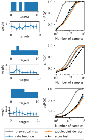
\includegraphics[]{figures/figure2.pdf}
  \caption{CGF network performance: change detection and adaptation. (Right) shows area under the ROC curve for a variety of label distributions (left, histograms) selected to show a variety of different performances. (Left, curves) show the average importance weights computed for members of each label.}
  \label{fig:2_change_detection}
\end{figure}

We apply these techniques to the simple case of a multilayer percepetron with one hidden layer of width 28, trained for classification of MNIST data.
Based on the activity of the hidden layer across all training points in the MNIST dataset, we train a CGF network and a conditional CGF network, which attain validation mean squared error of $\sim 0.04$ and $\sim 0.06$ respectively, indicating that they are, at minimum, fitting the eCGF reasonably well in the sampled regions.

First, we evaluate the performance of the CGF network model at distributional shift detection.
The task here is to detect changes in the frequencies of each target class in the MNIST test data. 
In Figure~\ref{fig:2_change_detection} on the right, we see a different change detection performances for several distribution shifts, chosen for their variety, some of which are more difficult than others.
The intrinsic difficulty of the change detection task naturally changes with how different the target distribution (histograms in Fig.~\ref{fig:2_change_detection} on the left) is from the uniform baseline that we are measuring relative to.
In Figure~\ref{fig:2_change_detection}, this intrinsic difficulty is show by the grey theoretical maximum curve, which corresponds to change detection by observing the ground-truth test set labels (which are not available to other methods).

In all of these cases, our rate function test achieves reasonable performance with hundreds of samples.
There is little difference between the performance of the rate function and the performance of the full saddlepoint density, and both of these are frequently similar to the score test.
This is particularly the case for the first and third tasks, one easy, in which some labels are never chosen, and one difficult, in which half of the label are chosen slightly more frequently than the other half.
The decreased performance of both rate function and score tests on these tasks may result from the cancellation of changes in the average activity, with multiple changes in label frequency balancing each other to produce only slight deviations in the mean.
The advantage of the rate function method shows up in the middle plots, corresponding to a single label that is more probable that the rest.
On this difficult task the rate function method performs quite well relative to the theoretical maximum, and significantly out-performs the score test.

Next, we evaluate the importance weights that are produced by exponential tilting, Figure~\ref{fig:2_change_detection} left.
We sample 200 subsets of the test data, each consisting of 100 datapoints, with the distributions of targets as show in the histograms.
We condition on successful change detection by the rate function test (with a p-value of 5\%) for each subset, and, given that a change is detected, evaluate the corresponding importance weights for all datapoints in the training set.
Averaging across datapoints with the same target and across all sampled subsets, produces the mean importance weights show in the curves in Figure~\ref{fig:2_change_detection} on the left.
Note that lower probability of a given target value results in a lower importance weight on average and therefore lesser impact on any weighted finetuning, and vice verse for higher probabilities.
There is also a significant amount of variance in the resulting weights, with the population standard deviations shown in Figure~\ref{fig:2_change_detection}.
This variance is likely a result of the fact that the importance weights are based on features within the classifier network, not purely the outputs, and therefore inputs with similar features but different labels will still be impacted.



\begin{figure}[tb]
  \centering
  \begin{subfigure}[t]{0.5\textwidth}
    \centering
    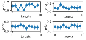
\includegraphics[]{figures/figure3a.pdf}
    \caption{Label distributions fit by prior regression for the three label distributions of Figure~\ref{fig:2_change_detection}, and a uniform label distribution (bottom right)}
    \label{fig:3a_prior_regression}
  \end{subfigure}
  \begin{subfigure}[t]{0.5\textwidth}
    \centering
    \includegraphics[]{figures/figure3b.png}
    \caption{Bayesian inference from conditional CGF: accuracy}
    \label{fig:3b_accuracy}
  \end{subfigure}
  \caption{Conditional CGF network: (a) results of prior regression to determine label distributions, (b) accuracy of Bayesian inference from hidden layer activity.}
  \label{fig:3_condtional_cgf}
\end{figure}

Finally, we evaluate the performance of the conditional CGF network for label shift detection and adaptation.
First, we compute the the sampling distribution over target labels by prior regression, fitting observed means as a linear combination of label-conditional means.
We show the resulting fit distributions in Figure~\ref{fig:3a_prior_regression} for each of the three label distributions from Figure~\ref{fig:2_change_detection}, as well as for the uniform case, in the bottom right plot.
We fit the label distributions for 200 samples of 100 datapoints each from each of the label distributions, plotting the mean and standard deviation of the recovered probabilities across samples. 
The fits are fairly accurate, clearly capturing the large label shifts in the top two plots, although with some small scale deviations between label values and a good amount of variance across samples.
We also evaluate the performance of Bayesian inference, using the conditional CGF networks to determine posterior label probabilities directly from the hidden layer activity. 
In Figure~\ref{fig:3b_accuracy} we show the accuracy of maximum a posteriori label decoding for uniform labels and each of the shifted label distributions.
The uniform case achieves about 84\% accuracy, which is reasonable, but significantly lower than the 96\% test performance achieved by classifier network as a whole.
The other label distributions achieve slightly higher MAP accuracy, likely due to their more concentrated priors.


\section{Discussion and Conclusion}

In this work, we have outlined a novel, principled approach to neural network distributional shift detection and adaptation, and demonstrated it in the simple case of MNIST label shifts.
However, the approach is not limited to label shifts: rate-function change detection and exponentially tilted fine-tuning are applicable to arbitrary distributional shifts.
Throughout this work, we have taken both the activity function of the classifier network, $T(x)$, and the label-to-parameter mapping, $\theta(y)$, to be fixed: learned and a simple heuristic, respectively.
This represents an important avenue for improvement: simultaneous training of these quantities together with the CGF network to produce a fully learned exponential family of distributions.
Paralleling variational autoencoders \cite{kingma_auto-encoding_2013}, which learn an \textit{outer approximation} to inference (approximate inference with specified noise and latent distributions), this direction resembles an \textit{inner approximation} to inference: exact inference with approximate distributions.
Finally, all of the procedures that we applied here can be applied to multiple hidden layers of a neural network simultaneously, producing sophisticated and learnable adaptation approaches.


\section{Models and methods}

Code for these models is available on github: \texttt{placeholder}

\subsection{CGF Network} \label{sec:network_architecture}

The CGF network is an input convex neural network \cite{amos_input_2017}, with convex non-linearities and positive weights after the first layer.
We use a multi-layer perceptron with no skip connections, but with positive weight matrices initialized as in \cite{hoedt_principled_2023}, and guaranteed to be positive by a ReLU applied to the weights.
For non-linearities, we use a leaky version of a softplus, given by $sp_{\textrm{leaky}}(x) = \alpha x + (1 - \alpha) sp(x) + c_0$ where $sp(x)$ is a softplus function, $\alpha$ sets the leak slope for negative values, and $c_0$ sets the intercept. 
These values are set to $\alpha =0.05$ and $c_0 = -0.693$, which sets the intercept to be the origin.
We choose the leaky softplus because it is convex (as required) and continuously differentiable, giving smooth Jacobians and Hessians, while retaining the benefits of leaky ReLUs in preventing dead units.
Additionally, it allows negative values to pass through the network, which is particularly important in the ICNN case, where the network weights are constrained to be positive.
We use three hidden layers, with widths of 200.

We generate the values of $\theta$ for the training set by sampling vectors with uniform orientations and lengths that are distributed according to a $\chi_1$ distribution, analogous to a univariate normal distribution.
The scale of the length distribution is set to $\sqrt{5}$.
This sampling method ensures that our samples are concentrated around the origin regardless of dimensionality, avoiding the well-known issue with high-dimensional multivariate normal distributions.
We find that about $10^6$ sample $\theta$ values are sufficient to achieve good fits to the eCGF.


We preprocess the activity data used as input to our CGF networks by removing the mean, and dividing by the variance across all dimension.
That is to say, we evaluate the mean $m = \frac{1}{n} \sum_i T_i$ and the variance ${v = \frac{1}{n}\sum_{ij} \left(T_{ij} - \frac{1}{n}\sum_{ij} T_{ij} \right)^2}$ of the training data, and transform all data $D$ to
\begin{equation}
  D_{\textrm{post}} = (D - m) /\sqrt{v}
\end{equation}
Note that $v$ is the \textit{scalar variance} across all dimensions of the data.
We use this method to produce centralized data without changing the structure or the relative importance of any dimension.

We perform dual optimization by gradient descent. We observed that different optimization hyper-parameters are better for different contexts.
Adam with small learning rate performs better in high dimensions, while SGD with momentum and large learning rate is preferable in lower dimensions.
This could be optimized by a hyper-parameter screen, but we stick to hand-tuning for the results in this paper.
Note that new data can be generated for dual evaluation, with the Jacobian of the forward model providing a means of evaluating the quality of the outputs.




\subsection{Model MNIST networks} \label{sec:model_network_details}

The MNIST network is a multilayer perceptron with one hidden layer and layer widths (784, 28, 10).
We train on the MNIST training data from the library \texttt{torchvision} with an 95\%-5\% train-validation split and early stopping.
This model achieves 96\% test accuracy.








\section*{Acknowledgements}

\texttt{Placeholder}

\section*{Impact Statement}
This paper presents work whose goal is to advance the field of 
Machine Learning. There are many potential societal consequences 
of our work, none which we feel must be specifically highlighted here.




\bibliography{main.bib}
\bibliographystyle{icml2025}

\end{document}